\documentclass{beamer}
\usepackage{listings}
\lstset{
%language=C,
frame=single, 
breaklines=true,
columns=fullflexible
}
\usepackage{blkarray}
\usepackage{subcaption}
\usepackage{url}
\usepackage{tikz}
\usepackage{tkz-euclide} % loads  TikZ and tkz-base
%\usetkzobj{all}
\usetikzlibrary{calc,math}
\usepackage{float}
\newcommand\norm[1]{\left\lVert#1\right\rVert}
\renewcommand{\vec}[1]{\mathbf{#1}}
\usepackage[export]{adjustbox}
\usepackage[utf8]{inputenc}
\usepackage{amsmath}
\usepackage{tikz}
\usepackage{hyperref}
\usepackage{bm}
\hypersetup{
    colorlinks = true,
    linkbordercolor = {white},
    linkcolor={red},
    citecolor={green},
    filecolor={blue},
	menucolor={red},
	runcolor={cyan},
	urlcolor={blue},
	breaklinks=true
}
\usetikzlibrary{automata, positioning}
\usetheme{Boadilla}
\providecommand{\pr}[1]{\ensuremath{\Pr\left(#1\right)}}
\providecommand{\mbf}{\mathbf}
\providecommand{\qfunc}[1]{\ensuremath{Q\left(#1\right)}}
\providecommand{\sbrak}[1]{\ensuremath{{}\left[#1\right]}}
\providecommand{\lsbrak}[1]{\ensuremath{{}\left[#1\right.}}
\providecommand{\rsbrak}[1]{\ensuremath{{}\left.#1\right]}}
\providecommand{\brak}[1]{\ensuremath{\left(#1\right)}}
\providecommand{\lbrak}[1]{\ensuremath{\left(#1\right.}}
\providecommand{\rbrak}[1]{\ensuremath{\left.#1\right)}}
\providecommand{\cbrak}[1]{\ensuremath{\left\{#1\right\}}}
\providecommand{\lcbrak}[1]{\ensuremath{\left\{#1\right.}}
\providecommand{\rcbrak}[1]{\ensuremath{\left.#1\right\}}}
\providecommand{\abs}[1]{\vert#1\vert}

\title{CSIR-UGC NET-Dec 2015-Problem(109)}
\author{Chirag Mehta}
\date{AI20BTECH11006}
\begin{document}

\begin{frame}
\titlepage
\end{frame}
\begin{frame}
\frametitle{Multivariate gaussian}
\begin{block}{Multivariate Gaussian expression, definition}
The multivariate normal distribution of a $n$ dimensional vector $\boldsymbol{X}=\brak{X_1,X_2,...,X_n}^\top$ can be written as
\begin{align}
f_{\boldsymbol{X}}(x_1,x_2,...,x_n)=\frac{\text{exp}\brak{-\frac{1}{2}\brak{\boldsymbol{x-\mu}}^\top\boldsymbol{\Sigma}^{-1}\brak{\boldsymbol{x-\mu}}}}{\sqrt{(2\pi)^2\abs{\boldsymbol{\Sigma}}}}
\end{align}
Mean vector $\boldsymbol{\mu}$ is defined as
\begin{align}
\boldsymbol{\mu}=E\sbrak{\boldsymbol{X}}=\brak{E\sbrak{X_1},E\sbrak{X_2},...,E\sbrak{X_n}}^\top
\end{align}
Covariance matrix $\boldsymbol{\Sigma}$ is defined as
\begin{align}
\Sigma_{i,j}=\text{Cov}\brak{X_i,X_j}
\end{align}

\end{block}
\end{frame}


\begin{frame}
\frametitle{multivariate gaussian contd.}
\begin{block}{equivalence}
A random vector $\boldsymbol{X}=\brak{X_1,X_2,...,X_n}^\top$ has a multivariate gaussian distribution if it satifies\\
\begin{itemize}
\item For every linear combination $Y=a_1X_1+a_2X_2+...+a_nX_n$ of its components in normally distributed. That is for any vector $\boldsymbol{a}\in\mathbb{R}^n$, the random variable $Y=a^\top X$ has a univariate normal distribution
\end{itemize}
\end{block}
\begin{block}{marginal probability}
\begin{align}
f_X(x)=\int\limits_{-\infty}^{\infty}f_{XY}(x,y)\,dy
\end{align}
\end{block}
\end{frame}


\begin{frame}
\frametitle{dirac delta function}
\begin{block}{dirac delta function}
An important property of dirac delta function that will be used at multiple ocassions in this solution is
\begin{align}
\displaystyle\int\limits_{-\infty}^{\infty} f(x)\delta(x-a)dx=f(a) \label{eq:dirac}
\end{align}
\end{block}
\end{frame}

\begin{frame}
\frametitle{Question}
\begin{block}{CSIR-UGC NET-Dec 2015-Problem(109)}
Suppose
$\begin{pmatrix}
X\\
Y
\end{pmatrix}$ is a random vector such that the marginal distribution of $X$ and the marginal distribution of $Y$ are the same and each is normally distributed with mean 0 and variance 1. Then, which of the following conditions imply independence of $X$ and $Y?$
\begin{enumerate}
\item Cov$\brak{X,Y}=0$
\item $aX+bY$ is normally distributed with mean 0 and variance $a^2+b^2$ for all real $a$ and $b$
\item $\pr{X\le 0, Y\le0}=\frac{1}{4}$
\item $E\sbrak{e^{itX+isY}}=E\sbrak{e^{itX}}E\sbrak{e^{isY}}$ for all real $s$ and $t$
\end{enumerate}
\end{block}
\end{frame}

\begin{frame}
\frametitle{Solution}
Given $X\sim N\brak{0,1}, Y\sim N(0,1)$
\begin{enumerate}[<+->]
\item
\begin{align}
Cov(X,Y)=0\\
E\sbrak{XY}-E\sbrak{X}E\sbrak{Y}=0\\
E\sbrak{XY}=0\\
\displaystyle \int\limits_{-\infty}^{\infty} \int\limits_{-\infty}^{\infty}xyf_{XY}(x,y)\, dx\,dy=0
\end{align}
This doesn't imply independence. Counter example given below
\end{enumerate}
\end{frame}

\begin{frame}
\frametitle{Solution Contd.}
\begin{enumerate}[<+->]
\item
Lets consider a case where $X$ and $Y$ are dependent based on the following relation, $Y$ being independent of $K$
\begin{align}
X=KY \label{eq:case}
\end{align}
PMF for $K$ is given as
\begin{align}
p_K(k)=
\begin{cases}
\frac{1}{2} &k=1\\
\frac{1}{2} & k=-1\\
0 & \text{otherwise}
\end{cases}
\end{align}
\end{enumerate}
\end{frame}

\begin{frame}
\frametitle{Solution Contd.}
\begin{enumerate}
\item
A simulation is given below, Y is gaussian, then X also follows gaussian
\begin{figure}[H]
\centering
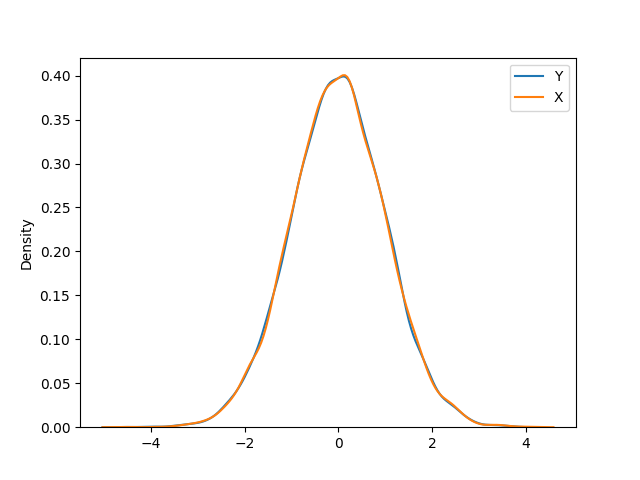
\includegraphics[width=.75\linewidth]{figure/fig}
\caption{X and Y, if Y is normal}
\label{plot}
\end{figure}
\end{enumerate}
\end{frame}

\begin{frame}
\frametitle{}
\begin{enumerate}\item
    Theoretically it can be proved in the following manner,
Since $K$ and $Y$ are independent
\begin{align}
f_X(x)&=\pr{K=1}f_Y(x)+\pr{K=-1}f_Y(-x)\\
&=\frac{1}{2}\brak{f_Y(x)+f_Y(-x)}\\
&=f_Y(x)
\end{align}
Therefore, $X$ follows identical but not independent distribution as $Y$, An alternative proof is given below as a proof for marginal probability
\end{enumerate}
\end{frame}

 \begin{frame}
 \frametitle{Solution Contd.}
\begin{enumerate}\item
Now consider that $X$ is normally distributed, we will establish $Y$ is also normally distributed.
The joint probability distribution is therefore
\begin{align}
f_{XY}(x,y)&=f_{X|Y}(x|y)f_X(x)\nonumber \\
&=f_X(x)\frac{1}{2}(\delta(x+y)+\delta(x-y))\label{eq:counter}
\end{align}
The marginal probability distribution function for $X$ is given as
\begin{align}
\int\limits_{-\infty}^{\infty}f_X(x)\frac{1}{2}(\delta(x+y)+\delta(x-y)) dy
\end{align}
Using \eqref{eq:dirac}, we get
\begin{align}
\int\limits_{-\infty}^{\infty}f_X(x)\frac{1}{2}(\delta(x+y)+\delta(x-y))dy=f_X(x)
\end{align}
We know that $X\sim N(0,1)$, $f_X(x)$ represents gaussian probability distribution function.
\end{enumerate}
\end{frame}

\begin{frame}
 \frametitle{Solution Contd.}
\begin{enumerate}\item
Futher, using symmetry of \eqref{eq:case}, we can establish that marginal distribution of $Y$ is gaussian. Here is a proof anyways
\begin{align}
f_Y(y)=\int\limits_{-\infty}^{\infty}f_X(x)\frac{1}{2}(\delta(x+y)+\delta(x-y)) dx
\end{align}
Using \eqref{eq:dirac}, we get
\begin{align}
f_Y(y)=\frac{1}{2}\brak{f_X(y)+f_X(-y)}=f_X(y)
\end{align}
Since $Y$ has identical probability distribution function, $Y\sim N(0,1)$
\end{enumerate}
\end{frame}
 
 \begin{frame}
 \frametitle{Solution Contd.}
\begin{enumerate}\item
 The covariance is given as
\begin{align}
&Cov(X,Y)=E[XY]-E[X]E[Y]=E[XY]\\
&E[XY]=\int\limits_{-\infty}^{\infty}\int\limits_{-\infty}^{\infty}xyf_{XY}(x,y)\, dy\, dx
\end{align}
\begin{align}
=\int\limits_{-\infty}^{\infty}\int\limits_{-\infty}^{\infty}xyf_X(x)\frac{1}{2}(\delta(x+y)+\delta(x-y))\,dy\,dx\\
=\int\limits_{-\infty}^{\infty} xf_X(x)\int\limits_{-\infty}^{\infty}y\frac{1}{2}(\delta(x+y)+\delta(x-y))\,dy\,dx
\end{align}
Using \eqref{eq:dirac}
\begin{align}
E[XY]=\int\limits_{-\infty}^{\infty}xf_X(x)\frac{1}{2}(x-x)\,dx=0
\end{align}
\end{enumerate}
 \end{frame}

 \begin{frame}
 \frametitle{Solution Contd.}
\begin{enumerate}
\setcounter{enumi}{1}
\item
Defining the following matrices/vectors
\begin{table}[h!]
\centering
\begin{tabular}{ |c|c|} 
\hline
\textbf{vector/matrix} & \textbf{expression} \\
\hline&\\[-1em]
$\boldsymbol{Z}$& $\begin{pmatrix} X &Y\end{pmatrix}^\top$\\[2pt]
\hline&\\[-1em]
$\boldsymbol{C}$&$\begin{pmatrix} a &b\end{pmatrix}^\top$  \\[2pt]
\hline&\\[-1em]
$\boldsymbol{\mu}$&$\begin{pmatrix} 0 &0\end{pmatrix}^\top$  \\[2pt]
\hline&\\[-1em]
$\boldsymbol{\Sigma}$&$\begin{pmatrix}1&\rho\\\rho&1\end{pmatrix}$ \\
\hline
\end{tabular}
\caption{vectors/matrices and their expressions}
\label{table1}
\end{table}
\end{enumerate}
 \end{frame}

 \begin{frame}
 \frametitle{Solution Contd.}
\begin{enumerate}
\setcounter{enumi}{1}
\item
Given
\begin{align}
\boldsymbol{C^\top Z}\sim N\brak{0,a^2+b^2}
\end{align}
Since this is true for all $a$ and $b$, it is equivalent to $X$ and $Y$ being jointly gaussian
\begin{align}
\boldsymbol{Z}\sim N(\boldsymbol{\mu},\boldsymbol{\Sigma})
\end{align}
For correlated random variables $X$ and $Y$ in bivariate normal distribution, we have
\begin{align}
\sigma_{Z}^2=\displaystyle\sum_{i,j}\Sigma_{ij}\\
a^2+b^2=a^2+b^2+2\rho ab\\
\therefore \rho=0\label{eq:rho}
\end{align}
\end{enumerate}
 \end{frame}

\begin{frame}
 \frametitle{Solution Contd.}
\begin{enumerate}
\setcounter{enumi}{1}
\item
The joint distribution is given as
\begin{align}
f_{\boldsymbol{Z}}(x,y)=\frac{\text{exp}\brak{-\frac{1}{2}\brak{\boldsymbol{z-\mu}}^\top\boldsymbol{\Sigma}^{-1}\brak{\boldsymbol{z-\mu}}}}{\sqrt{(2\pi)^2\abs{\boldsymbol{\Sigma}}}}\\
f_{\boldsymbol{Z}}(x,y)=\frac{\text{exp}\brak{-\frac{1}{2}{\begin{pmatrix} x &y\end{pmatrix}} I_2{\begin{pmatrix} x &y\end{pmatrix}}^\top}}{\sqrt{(2\pi)^2}}
\end{align}
Where $I_2$ is the identity matrix of order 2
\begin{align}
f_{\boldsymbol{Z}}(x,y)=\frac{\text{exp}\brak{-\frac{1}{2}{\begin{pmatrix} x &y\end{pmatrix}} {\begin{pmatrix} x &y\end{pmatrix}}^\top}}{\sqrt{(2\pi)^2}}\\
f_{\boldsymbol{Z}}(x,y)=\frac{\text{exp}\brak{-\frac{1}{2}\brak{x^2+y^2}}}{\sqrt{(2\pi)^2}}=f_X(x)f_Y(y)
\end{align}
$\therefore$ \textbf{Option(2) is correct}
\end{enumerate}
\end{frame}

\begin{frame}
 \frametitle{Solution Contd.}
\begin{enumerate}
\setcounter{enumi}{1}
\item
A simulation for bivariate gaussian is given below
\begin{figure}[H]
\centering
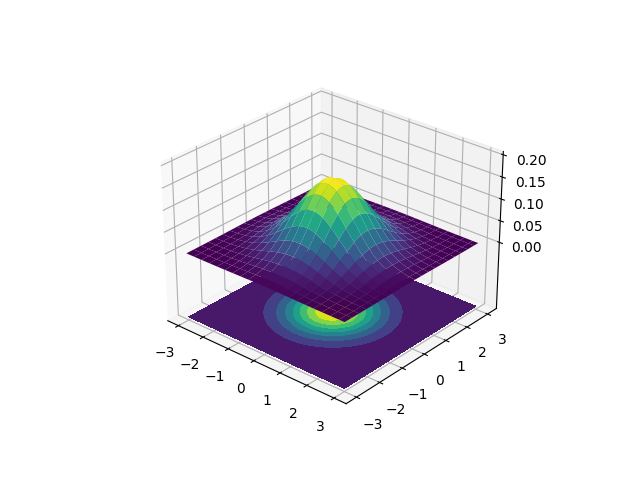
\includegraphics[width=0.75\linewidth]{figure/plot}
\caption{bivariate gaussian with 0 mean vector\\ and identity covariance matrix}
\label{plot}
\end{figure}
\end{enumerate}
\end{frame}

\begin{frame}
 \frametitle{Solution Contd.}
\begin{enumerate}
\setcounter{enumi}{2}
\item
\begin{align}
\pr{X\le 0, Y\le0}=\frac{1}{4}
\end{align}
This doesn't imply independence, it can be true even for dependent $X$ and $Y$, the counter example is \eqref{eq:counter}, the joint probability function is symmetric across all 4 quadrants
\begin{align}
\therefore \pr{X\le 0, Y\le0}=\frac{1}{4}
\end{align}
Alternatively, here is proof 
\begin{align}
\pr{X\le 0}=F_X(0)=\frac{1}{2} \label{eq:pr1}
\end{align}
Using \eqref{eq:case}
\begin{align}
\pr{Y\le 0|X\le 0}=\frac{1}{2} \label{eq:pr2}
\end{align}
\end{enumerate}
\end{frame}

\begin{frame}
 \frametitle{Solution Contd.}
\begin{enumerate}
\setcounter{enumi}{2}
\item
Using \eqref{eq:pr1} and \eqref{eq:pr2}
\begin{align}
\pr{X\le 0, Y\le0}=\frac{1}{4}
\end{align}
\item
\begin{align}
E\sbrak{e^{itX+isY}}=E\sbrak{e^{itX}}E\sbrak{e^{isY}}\\
E\sbrak{e^{itX+isY}}=\varphi_X(t)\varphi_Y(s) \label{eq:inde}
\end{align}
\end{enumerate}
\end{frame}

\begin{frame}
 \frametitle{Solution Contd.}
\begin{enumerate}\setcounter{enumi}{3}
\item
The inverse is given as
\begin{align}
f_{XY}(x,y)=\frac{1}{4\pi^2}\displaystyle \int\limits_{-\infty}^{\infty} \int\limits_{-\infty}^{\infty} e^{-itX-isY}E\sbrak{e^{itX+isY}}\,ds\,dt
\end{align}
Using \eqref{eq:inde}
\begin{align}
f_{XY}(x,y)&=\frac{1}{4\pi^2}\displaystyle \int\limits_{-\infty}^{\infty} \int\limits_{-\infty}^{\infty} e^{-itX-isY}\varphi_X(t)\varphi_Y(s)\,ds\,dt\\
&f_{XY}(x,y)=f_X(x)f_Y(y)
\end{align}
$\therefore$ \textbf{Option(4) is correct}
\end{enumerate}
\end{frame}

\begin{frame}
\frametitle{Reading material}
\begin{enumerate}
\item Sum of 2 gaussian random variables need not be gaussian\\
\url{https://github.com/planetmath/62_Statistics/blob/master/pdf/62E15-SumsOfNormalRandomVariablesNeedNotBeNormal.pdf}
\item Multivariate gaussian\\
\begin{itemize}
\item\url{https://bit.ly/2RComEB}\\
\item\url{https://en.wikipedia.org/wiki/Multivariate_normal_distribution}
\end{itemize}
\item Characteristic function of multivariate gaussian\\
\url{https://bit.ly/3gbWZeF}
\end{enumerate}
\end{frame}


\end{document}